\documentclass{article}
\usepackage{amsfonts}
\usepackage{amsmath}
\usepackage{amssymb}
\usepackage{amsthm}
\usepackage{centernot}
\usepackage{enumitem}
\usepackage{float}
% \usepackage[margin=1in]{geometry}
\usepackage{parskip}
\usepackage{pgfplots}
\usepackage{tikz}
\usepackage{titling}

\newcommand{\Z}{\mathbb{Z}}
\newcommand{\Q}{\mathbb{Q}}

\setcounter{section}{4}

% axis style, ticks, etc
\pgfplotsset{
  every axis/.append style={
    axis x line=middle,    % put the x axis in the middle
    axis y line=middle,    % put the y axis in the middle
    axis line style={<->}, % arrows on the axis
    xlabel={$x$},          % default put x on x-axis
    ylabel={$y$},          % default put y on y-axis
  }
}

% arrows as stealth fighters
\tikzset{>=stealth}

\begin{document}

\title{\vspace{-3cm}MTH 505 Homework 4}
\author{Roy Howie}
\date{April 14, 2017}
\maketitle

% problem 4.1
\subsection{Squares Mod 4}
  \begin{enumerate}[label=\textbf{(\alph*)}]
    \item{
      Note $0^2\equiv0$, $1^2\equiv1$, $2^2\equiv0$, and $3^2\equiv1$ modulo 4.
      Thus 0 and 1 are the only square elements of $\Z_4$.
    }
    \item{
      First, for $n\in\Z$, note $n\equiv1\pmod{2}$ implies $n^2\equiv1\pmod{4}$.
      Next, let $x,y,z\in\Z$ such that $x^2+y^2=z^2$. Suppose $x$ and $y$ are
      both odd, then $x^2\equiv y^2\equiv1\pmod{4}$, implying $z^2\equiv2
      \pmod{4}$. A contradiction, as 2 is not a square elements of $\Z_4$.
      Hence, $x$ and $y$ cannot both be odd.
      \qed
    }
  \end{enumerate}

% problem 4.2
\subsection{Fermat's Last Theorem}
  Consider (FLT): $x^4+y^4=z^2$ for $x,y,z\in\Z$ with $xyz\ne0$.
  \begin{enumerate}[label=\textbf{(\alph*)}]
    \item{
      Suppose FLT has a solution $(x_1,y_1,z_1)\in\Z^3$, then there is another
      solution $(x_n,y_n,z_n)\in\Z^3$ with $\gcd(x_n,y_n)=1$ and $0<z_n<|z|$.

      Let $p$ be a prime divisor of both $x_1$ and $y_1$. If no such number
      exists, then $\gcd(x_1,y_1)=1$ and we are done. Otherwise, $(x_1/p,y_1/p,
      z_1/p^2)$ is another solution, as $(x_1/p)^4+(y_1/p)^4=(x_1^4+y_1^4)/p^4=
      z_1^2/p^4$. Recurse.
    }
    \item{
      Suppose $(x,y,z)$ is a solution to FLT with $\gcd(x,y)=1$.

      Note $x$ and $y$ cannot both be odd, as $x^4+y^4=(x^2)^2+(y^2)^2=z^2$.
      WLOG, assume $x$ is odd, $y$ is even, and $z=|z|$. There are then coprime
      $u,v\in\Z$ with $v>0$ such that $x^2=v^2-u^2$, $y=2uv$, and $z=u^2+v^2$.
      As $u^2+x^2=v^2$, there are again coprime $r,s\in\Z$ with
      $s>0$ such that $x=s^2-r^2$, $u=2rs$, and $v=r^2+s^2$.

      Next, consider $y^2=2uv$. Since $y$ is even, 4 divides $y^2$. Note $u$
      is even, as $x$ is odd and $u^2+x^2=v^2$. Thus, $(y/2)^2=(u/2)v$. Recall
      $\gcd(u,v)=1$ and that if a prime $p$ divides a number $t^2$, then $p^2$
      does too. Therefore, if $p^2$ divides $(y/2)^2$, then $p^2$ divides either
      $u/2$ or $v$. Hence, $u/2$ and $v$ are perfect squares each. By similar
      argument, as $u=2rs$ and $u/2$ is an even square number, $r$ and $s$ are
      also perfect squares.

      Therefore, there are $(m,n,l)\in\Z^3$ with $s=m^2$, $r=n^2$, and $v=l^2$.
      Note $v=r^2+s^2$, so $l^2=m^4+n^4$ and $(m,n,l)$ is another solution to
      FLT. Furthermore, $\gcd(m,n)=1$, as$r$ and $s$ were coprime; $mnl\ne0$, as
      $rsv\ne0$, and $0<l<|z|$, as $z=u^2+v^2$ with $v$ positive and $v=l^2$.

      We are back to square one, contradicting the well ordering of the
      integers, as every solution $(a,b,c)$ to FLT produces another solution
      $(d,e,f)$ with $0<f<|c|$. Hence, no solution to FLT exists.
      \qed
    }
  \end{enumerate}

% problem 4.3
\subsection{Rational Points on a Hyperbola}
  Consider (Hyp): $4\alpha^2-4\alpha\beta-7\beta^2-16\beta-12=0$.
  \begin{enumerate}[label=\textbf{(\alph*)}]
    \item{
      Let $P=\left(\begin{smallmatrix}1&0.5\\0&1\end{smallmatrix}\right)$ and
      $u=(-0.5,-1)$. Apply the affine transformation $x=Px'+u$, where $x=(\alpha,
      \beta)$ and $x'=(x,y)$. This yields $\alpha=x+0.5y-0.5$ and $\beta=y-1$.
    }
    \item{
      \begin{figure}[H]
        \hspace*{1cm}
        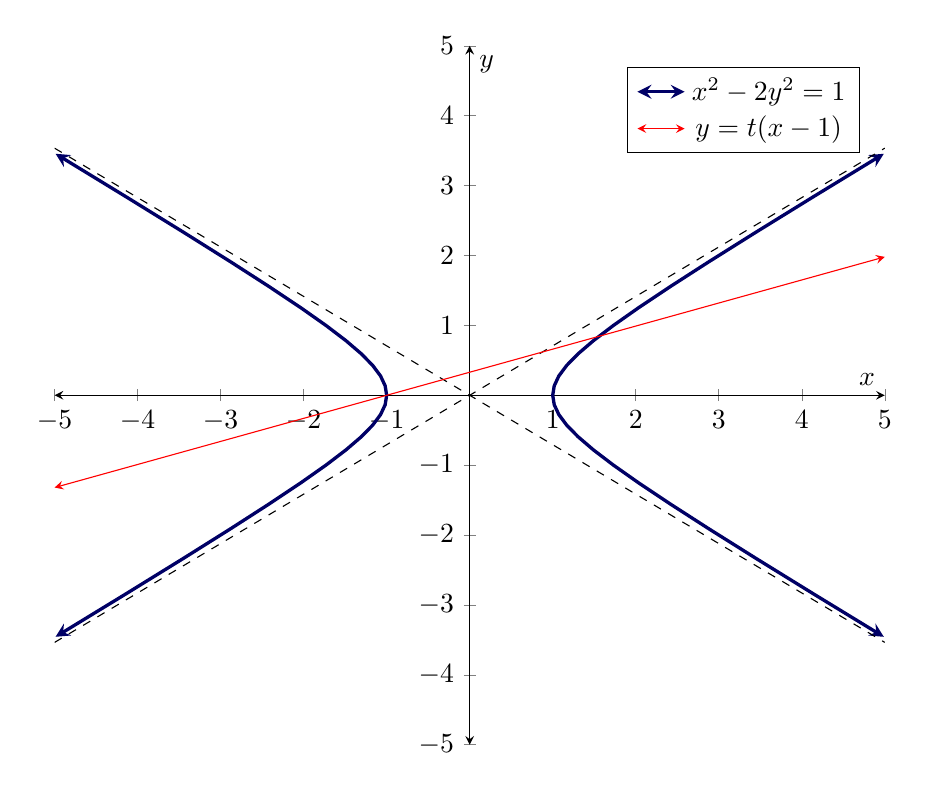
\begin{tikzpicture}
          \begin{axis}[
              xmin=-5,xmax=5,
              ymin=-5,ymax=5,
              legend pos=north east,
              width=\textwidth,
            ]
            \addplot [blue!40!black,very thick,domain=-2.29:2.29,<->]
              ({cosh(x)}, {sinh(x)/sqrt(2)});
            \addplot [blue!40!black,very thick,domain=-2.29:2.29,<->]
              ({-cosh(x)}, {sinh(x)/sqrt(2)});
            \addplot[black,dashed] expression {+x/sqrt(2)};
            \addplot[black,dashed] expression {-x/sqrt(2)};
            \addplot[red,<->,domain=-5:5] expression {0.33*(x+1)};
            \legend{$x^2-2y^2=1$,,,,$y=t(x-1)$}
          \end{axis}
        \end{tikzpicture}
      \end{figure}
    }
    \item{
      Consider the equations $x^2-2y^2=1$ and $y=t(x+1)$, then
      \begin{align*}
        0 &= x^2-2y^2-1\\
          &= x^2-2t^2(x+1)^2-1\\
          &= x^2\underbrace{(1-2t^2)}_a+x\underbrace{(-4t^2)}_b+
            \underbrace{(-2t^2-1)}_c
      \end{align*}
      Using the quadratic formula gives
      \begin{align*}
        x &= \frac{-b\pm\sqrt{b^2-4ac}}{2a}\\
          &= \frac{4t^2\pm\sqrt{16t^2+4(1-2t^2)(2t^2-1)}}{2(1-2t^2)}\\
          &= \frac{4t^2\pm2}{2(1-2t^2)}\\
          &=-1\text{\quad or\quad}\frac{1+2t^2}{1-2t^2}\\
      \end{align*}
      Substituting $x$ into $y=t(x+1)$ yields
      \begin{align*}
        y = t(x+1)
          = t\left(\frac{1+2t^2}{1-2t^2}+1\right)
          = \frac{2t}{1-2t^2}
      \end{align*}
      Thus, $(x_t,y_t)=\left(\frac{1+2t^2}{1-2t^2},\frac{2t}{1-2t^2}\right)$ for
      $t\ne\pm1/\sqrt{2}$.

      Clearly, $t\in\Q\iff(x_t,y_t)\in\Q^2$.
    }
    \item{
      Substituting $t=u/v$ for coprime $u,v\in\Z$ with $v>0$ into $(x_t,y_t)$
      produces
      \begin{align*}
        x_t
          &= \frac{1+2t^2}{1-2t^2}
          = \frac{1+2\left(\frac{u}{v}\right)^2}{1-2\left(\frac{u}{v}\right)^2}
          = \frac{2u^2+v^2}{v^2-2u^2}\\
        y_t
          &= \frac{2t}{1-2t^2}
          = \frac{2\left(\frac{u}{v}\right)^2}{1-2\left(\frac{u}{v}\right)^2}
          = \frac{2uv}{v^2-2u^2}\\
      \end{align*}
    }
    \item{
      Inverting the affine transformation presented in \textbf{4.4.3a} gives
      $x'=P^{-1}(x-u)$, or that $x=\alpha-\beta/2$ and $y=\beta+1$. Thus,
      \begin{align*}
        \alpha &= \frac{2u^2+v^2}{v^2-2u^2}+\frac{uv}{v^2-2u^2}-\frac{1}{2}\\
        \beta &= \frac{2uv}{v^2-2u^2}-1
        \tag*{\qed}
      \end{align*}
    }
  \end{enumerate}

% problem 4.4
\subsection{A Hyperbola with No Rational Points}

\end{document}
